\documentclass[border=10pt]{standalone}
%%%<
\usepackage{verbatim}
%%%>
\usepackage{pgfplots}
\pgfplotsset{width=7cm,compat=1.8}
\begin{comment}
:Title: Surface plot with interior colors
:Tags: 3D;Surface plots;Manual
:Author: Christian Feuersänger
:Slug: surface-interior-color

A surface plot visualizes a two dimensional, single patch using
different fill colors for each patch segment.
Each patch segment is a (pseudo) rectangle, that means input data
is given in form of a data matrix.

We can distinguish between the outer side and the interior
parts of a surface by choosing different colors.

The code is from the PGFPlots 1.10 manual: "4.6.6 Surface Plots".
\end{comment}
\begin{document}
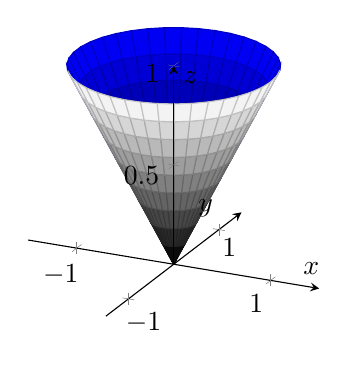
\begin{tikzpicture}
\begin{axis}[
  axis lines=center,
  axis on top,
  xlabel={$x$}, ylabel={$y$}, zlabel={$z$},
  domain=0:1,
  y domain=0:2*pi,
  xmin=-1.5, xmax=1.5,
  ymin=-1.5, ymax=1.5, zmin=0.0,
  mesh/interior colormap=
  	{blueblack}{color=(black) color=(blue)},
  colormap/blackwhite, 
  samples=10,
  samples y=40,
  z buffer=sort,
 ]
  \addplot3[surf] 
  	({x*cos(deg(y))},{x*sin(deg(y))},{x});
\end{axis}
\end{tikzpicture}
\end{document}
